\setcounter{subsection}{-1}

% s~s~s~s~s~s~s~s~s~s~s~s~s~s~s~s~s~s~s~s~s~s~s~s~s~s~s~s~s~s~s~s~s~s~s~s~s~s~s~s~s~s~s~s
% s~s~s~s~s~s~s~s~s~s~s~s~s~s~s~s~s~s~s~s~s~s~s~s~s~s~s~s~s~s~s~s~s~s~s~s~s~s~s~s~s~s~s~s
\subsection{Wolfram Alpha Syntax (optional)}
You may want to use Wolfram Alpha (wolframalpha.com) to check your answers. If you're not sure what syntax to use to compute double integrals with Wolfram Alpha, let's suppose that we want to determine the value of
\begin{align*} 
   \mathop{\int_{-2}^{-1} \!  \int_0^{x-1}}( x^{2C} +y)  dy  dx
\end{align*}
where $C$ is a constant. The syntax we could use to compute this particular integral is
\begin{quote}
  \begin{verbatim}
    integrate x^{2C}+y dydx, x from -2 to -1 and y from 0 to (x-1)
  \end{verbatim}
\end{quote}
% END OF SUBSECTION
% s~s~s~s~s~s~s~s~s~s~s~s~s~s~s~s~s~s~s~s~s~s~s~s~s~s~s~s~s~s~s~s~s~s~s~s~s~s~s~s~s~s~s~s
% s~s~s~s~s~s~s~s~s~s~s~s~s~s~s~s~s~s~s~s~s~s~s~s~s~s~s~s~s~s~s~s~s~s~s~s~s~s~s~s~s~s~s~s
\subsection{Double Integrals}
\purple{\From Section 3.1 of \VCT.}

\BEN
% ~~~~~~~~~~~~~~~~~~~~~~~~~~~~~~~~~~~~~~~~~~~~~~~~~~~~~~~~~~~~~~~~~~~~~~~~~~~~~~~~~
\item % VOLUME OF SIMPLE SOLID 
Consider the solid that lies under the plane $z = -x-2y+2$ and above the rectangle \\$\{(x,y) \ | \ -2\le x\le 0, 0\le y \le1 \}$.
\BEN
\item Sketch the solid in $\R^3$. \textit{Hint: start by plotting the points that are located on the given plane and above the corners of the rectangle. Then connect the points with solid lines.}
\item Find the volume of the solid.
\EEN
% ~~~~~~~~~~~~~~~~~~~~~~~~~~~~~~~~~~~~~~~~~~~~~~~~~~~~~~~~~~~~~~~~~~~~~~~~~~~~~~~~~
\item % FLUID MECHANICS
\textbf{Application to Fluid Mechanics} \\
In a two-dimensional, steady-state, incompressible fluid flow, the velocity \textbf{v} of the flow can be expressed as $\MB{v} = u(x,y)\MB{i} + v(x,y)\MB{j}$. The functions $u(x,y)$ and $v(x,y)$ must satisfy 
\begin{align*}
  \nabla\cdot\MB{v} = 0.
\end{align*}
\BEN
\item If $u(x,y) = x^2 + y^2$, find the most general form of $v(x,y)$. 
\item If $v(x,y) = \cos(x)$, find the most general form of $u(x,y)$.
\EEN
\textit{Hint: you are asked to find the most \Emph{general} form of functions u and v}.

\EEN % END OF SUBSECTION
% s~s~s~s~s~s~s~s~s~s~s~s~s~s~s~s~s~s~s~s~s~s~s~s~s~s~s~s~s~s~s~s~s~s~s~s~s~s~s~s~s~s~s~s
% s~s~s~s~s~s~s~s~s~s~s~s~s~s~s~s~s~s~s~s~s~s~s~s~s~s~s~s~s~s~s~s~s~s~s~s~s~s~s~s~s~s~s~s
\subsection{Double Integrals Over a General Region}
\purple{\From Section 3.2 of \VCT.}

\BEN
% ~~~~~~~~~~~~~~~~~~~~~~~~~~~~~~~~~~~~~~~~~~~~~~~~~~~~~~~~~~~~~~~~~~~~~~~~~~~~~~~~~
\item % TETRAHEDRON
\Emph{Volume of a Tetrahedron} \\
A \Emph{tetrahedron} is a three dimensional object with four, triangular, flat sides. Because each of its four sides are flat, a tetrahedron can be defined as the region enclosed by four planes. Below is a sketch of two tetrahedrons. Note that each tetrahedron has four vertices, six edges, and that the lengths of its edges do not have to be equal.
\begin{figure}[h]
  \vspace{-1pt}
  \begin{center}
    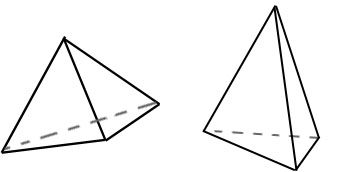
\includegraphics[width=0.35\textwidth]{ImgTetrahedrons.jpg}
  \end{center}
\end{figure}\\
Consider the tetrahedron that is bounded by the three coordinate planes in $\R^3$, and by the plane $z = 1 - x - \frac{y}{2}$.
\BEN
\item Sketch the tetrahedron in $\R^3$ and label the points that represent its four vertices. 
\item Set up, but do not evaluate, a double integral that represents the volume of the tetrahedron. Integrate with respect to $x$ first. 
\item Set up, but do not evaluate, a double integral that represents the volume of the tetrahedron. Integrate with respect to $y$ first. 
\EEN
Note that
\begin{itemize}
\item Examples 3.4 and 3.5 from \VCT \ are similar to this problem. 
\item We could also calculate the volume of the solid by using a \Emph{triple} integral. 
\item Although not required, the double integrals are straightforward to compute. You may want to check your answers by evaluating the integrals and seeing if you would get the same result in parts (b) and (c). 
\end{itemize}
% ~~~~~~~~~~~~~~~~~~~~~~~~~~~~~~~~~~~~~~~~~~~~~~~~~~~~~~~~~~~~~~~~~~~~~~~~~~~~~~~~~
\item  % DESCRIBE WHY A PARTICULAR DOUBLE INTEGRAL GIVES AREA
\Emph{Area of a General Region}
\BEN
\item Question 11 from Section 3.2 of \VCT. \textit{Hint: Figure 3.2.5 is also helpful.}
\item Use the result from part (a) to compute the area of the region bounded by the curves $y = x^2$ and $x=y^2$.
\EEN

% ~~~~~~~~~~~~~~~~~~~~~~~~~~~~~~~~~~~~~~~~~~~~~~~~~~~~~~~~~~~~~~~~~~~~~~~~~~~~~~~~~
\item % UPPER AND LOWER BOUNDS ARE FUNCTIONS
Find the volume of the solid enclosed by $z = x^2 + y^2$, $y = x^2$ and $x=y^2$.
% ~~~~~~~~~~~~~~~~~~~~~~~~~~~~~~~~~~~~~~~~~~~~~~~~~~~~~~~~~~~~~~~~~~~~~~~~~~~~~~~~~
\item % CHANGING ORDER OF INTEGRATION
Consider the integral
\begin{align*}
  \iint\limits_R x\sin(y) dA
\end{align*}
 where $R$ is the region bounded by $y=0$, $y=x^2$, and $x=2$.
\BEN
\item Evaluate the double integral by first integrating with respect to $x$. 
\item Evaluate the double integral by first integrating with respect to $y$. 
\EEN
Note that your answers for both parts should be the same, and that you may need to use various techniques of integration to complete this problem, including integration by parts and a variable substitution. 
% ~~~~~~~~~~~~~~~~~~~~~~~~~~~~~~~~~~~~~~~~~~~~~~~~~~~~~~~~~~~~~~~~~~~~~~~~~~~~~~~~~
\item % CHANGING ORDER OF INTEGRATION, GENERAL F(X,Y)
Consider the double integral
\begin{align*}
  \mathop{\int_{0}^{1+e} \! \int_0^{\ln(x-1)}} f(x,y) dydx .
\end{align*}
Sketch the region in $\R^2$ over which $f(x,y)$ is integrated, and change the order of integration.  
% ~~~~~~~~~~~~~~~~~~~~~~~~~~~~~~~~~~~~~~~~~~~~~~~~~~~~~~~~~~~~~~~~~~~~~~~~~~~~~~~~~
\item % BOUNDING AN INTEGRAL 
Consider the double integral
\begin{align*}
  \iint\limits_D f(x,y) dA,
\end{align*}
where $D$ is the square $0\le x \le 1$, $0\le y \le 1$, and $f(x,y) = \sin(x+y)$. Show that 
\begin{align*}
  0 \le \iint\limits_D f(x,y) dA \le 1.
\end{align*}
% ~~~~~~~~~~~~~~~~~~~~~~~~~~~~~~~~~~~~~~~~~~~~~~~~~~~~~~~~~~~~~~~~~~~~~~~~~~~~~~~~~
\item % SYMMETRY
\textbf{Simplifying Double Integrals Using Symmetry} \\
Certain integrals can be simplified when the integrand is either even or odd. You may know that, for functions of one variable, that
\begin{align*}
  \text{if }f(x)\text{ is odd, then } & \int_{-a}^{a} f(x) dx = 0 . \\
  \text{if }f(x)\text{ is even, then } & \int_{-a}^{a} f(x) dx = 2 \int_0^a f(x) dx.
\end{align*}
There are similar results for integrals of two variables, but in order to introduce them, we first need to extend our concepts of even and odd functions to functions of two variables, and we need to describe regions that are symmetric about the $x$-axis and about the $y$-axis. 

If $R$ is a region that is \Emph{symmetric about the $y$-axis}, and $(x_0,y_0)$ is a point inside $R$, then the point $(-x_0,y_0)$ is also inside $R$. Similarily, if $S$ is a region that is \Emph{symmetric about the $x$-axis}, and $(x_1,y_1)$ is a point inside $S$, then the point $(x_1,-y_1)$ is also inside $S$. Above are examples of regions that have these symmetries.\\

\begin{figure}[h]
  \vspace{-1pt}
  \begin{center}
    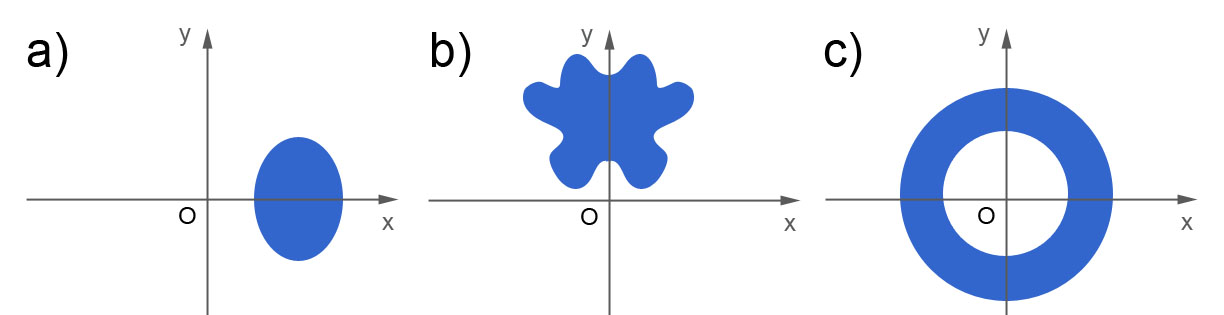
\includegraphics[width=0.95\textwidth]{ImgRegions.jpg}
  \end{center}
 \begin{quote} \caption{\small{a) the blue region is symmetric about the $x$-axis, b) the blue region is symmetric about the $y$-axis, and c) the blue region is symmetric about the $x$-axis and the $y$-axis.}}\end{quote}
\end{figure}

Moreover, if $g(x,y)$ is odd in $x$, then 
\begin{align*}
  g(-x,y) = - g(x,y).
\end{align*}
But if $g(x,y)$ were even in $x$, then 
\begin{align*}
  g(-x,y) =  g(x,y).
\end{align*}
Combining these concepts yields helpful results for computing double integrals. For example, if $R$ is symmetric about the $y$-axis, and if $g(x,y)$ is odd in $x$, then
\begin{align*}
  \iint\limits_R g(x,y) dxdy = 0.
\end{align*}
Similar results can be stated if $g$ were even in $x$ or in $y$, and if $R$ has symmetry about the $x$-axis. 
\BEN
\item Provide an example of a non-zero function of two variables, $h(x,y)$, that is odd in $x$. Verify that your function is odd in $x$.
\item Provide an example of a region, $D$, that is symmetric about the $y$-axis, but is not symmetric about the $x$-axis. 
\item Show that, for your $h(x,y)$ and region $D$, that 
\begin{align*}
  \iint\limits_D g(x,y) dxdy = 0.
\end{align*}
\EEN

\EEN % END OF SUBSECTION
% s~s~s~s~s~s~s~s~s~s~s~s~s~s~s~s~s~s~s~s~s~s~s~s~s~s~s~s~s~s~s~s~s~s~s~s~s~s~s~s~s~s~s~s
% s~s~s~s~s~s~s~s~s~s~s~s~s~s~s~s~s~s~s~s~s~s~s~s~s~s~s~s~s~s~s~s~s~s~s~s~s~s~s~s~s~s~s~s

\subsection{Triple Integrals}
\purple{\From Section 3.3 of \VCT.}
  
\BEN
% ~~~~~~~~~~~~~~~~~~~~~~~~~~~~~~~~~~~~~~~~~~~~~~~~~~~~~~~~~~~~~~~~~~~~~~~~~~~~~~~~~
\item % TETRAHEDRON
\Emph{Volume of a Tetrahedron} \\
The textbook points out that the triple integral 
\begin{align*}
  \iiint\limits_S f(x,y,z) dV
\end{align*}
for the special special case when $f(x,y,z) = 1$ for all points in $S$, gives the volume of $S$
\begin{align*}
  V(S) &= \iiint\limits_S dV.
\end{align*}
Consider again the tetrahedron that is bounded by the three coordinate planes in $\R^3$, and by the plane $z = 1 - x - \frac{y}{2}$. We derived an expression for the volume of this tetrahedron in a previous question using a double integral. Now set-up and find the volume of the tetrahedron using a triple integral.
% ~~~~~~~~~~~~~~~~~~~~~~~~~~~~~~~~~~~~~~~~~~~~~~~~~~~~~~~~~~~~~~~~~~~~~~~~~~~~~~~~~
\item % VOLUME OF AN ELLIPSOID
\textbf{Volume of an Ellipsoid}\\
Solve Question 10 from Section 3.5 of \VCT.
% ~~~~~~~~~~~~~~~~~~~~~~~~~~~~~~~~~~~~~~~~~~~~~~~~~~~~~~~~~~~~~~~~~~~~~~~~~~~~~~~~~
\item % VOLUME OF SOLID
\textbf{Volume of a Solid}\\
Find the volume of the solid enclosed by the planes
\begin{align*}
  z & = x+y\\
  y &= x \\
  x &= 0 \\
  z &= -1 \\
  y &= 2
\end{align*}
\textit{Hint: it may help to start by plotting the planes in Google or in Wolfram Alpha.}\\
\rednote{The solutions need to be adjusted so that z is in -1 to x+y}
\EEN % END OF SUBSECTION
% s~s~s~s~s~s~s~s~s~s~s~s~s~s~s~s~s~s~s~s~s~s~s~s~s~s~s~s~s~s~s~s~s~s~s~s~s~s~s~s~s~s~s~s
% s~s~s~s~s~s~s~s~s~s~s~s~s~s~s~s~s~s~s~s~s~s~s~s~s~s~s~s~s~s~s~s~s~s~s~s~s~s~s~s~s~s~s~s
\subsection{Change of Variables in Multiple Integrals}
\purple{\From Section 3.5 of \VCT.}
\BEN
% ~~~~~~~~~~~~~~~~~~~~~~~~~~~~~~~~~~~~~~~~~~~~~~~~~~~~~~~~~~~~~~~~~~~~~~~~~~~~~~~~~
\item % GENERAL TRANSFORMATION
\Emph{Linear Transformations} \\
Under the linear transformation 
\begin{align*}
  x = c_1u + c_2v , \quad y =d_1u + d_2v, \quad d_1c_2 - d_2c_1 \ne 0,
\end{align*}
straight lines in the $uv$-plane are mapped to straight lines in the $xy$-plane. 
\BEN
\item $v=v_0$ is a horizontal line in the $uv$-plane. Determine the equation of this line in the $xy$-plane. 
\item $x=x_0$ is a vertical line in the $xy$-plane. Determine the equation of this line in the $uv$-plane.
\EEN
% ~~~~~~~~~~~~~~~~~~~~~~~~~~~~~~~~~~~~~~~~~~~~~~~~~~~~~~~~~~~~~~~~~~~~~~~~~~~~~~~~~
\item % STRAIGHTFORWARD CHANGE OF VARIABLES
Use an appropriate transformation to evaluate the integral
\begin{align*}
  \iint\limits_R \big(x^2 - y^2\big) dxdy,
\end{align*}
where $R$ is the parallelogram bounded by 
\begin{align*}
  x+y = 0, \quad x+y = 1, \quad x-y=0, \quad x-y=1.
\end{align*}

% ~~~~~~~~~~~~~~~~~~~~~~~~~~~~~~~~~~~~~~~~~~~~~~~~~~~~~~~~~~~~~~~~~~~~~~~~~~~~~~~~~
\item % CHANGE OF VARIABLES TWICE
\Emph{Simplifying Double Integrals} \\
When working with double integrals over a rectangular region $R=\{(x,y) | a \le x \le b, c\le y \le d\}$, we can use the simplification
\begin{align*}
   \iint\limits_{R} g(x) h(y) dA 
  & = \int_a^b g(x) dx \int_c^d h(y) dy  
\end{align*}
Use this property and the transformation $x = 3u, y = 2v$ to evaluate the double integral
\begin{align*}
  \iint\limits_E x^2 \ dxdy,
\end{align*}
where $E$ is region bounded by the ellipse $4x^2 + 9y^2 = 36$. 
% ~~~~~~~~~~~~~~~~~~~~~~~~~~~~~~~~~~~~~~~~~~~~~~~~~~~~~~~~~~~~~~~~~~~~~~~~~~~~~~~~~
\item % SIMPLE CYLINDRICAL WITH CONE
Evaluate the integral
\begin{align*}
  \iiint\limits_S y^2dV,
\end{align*}
where $S$ is the solid that lies inside the cylinder $x^2+y^2 = 1$, above the plane $z=0$ and below the cone $z^2 = 9x^2 + 9y^2$. 
% ~~~~~~~~~~~~~~~~~~~~~~~~~~~~~~~~~~~~~~~~~~~~~~~~~~~~~~~~~~~~~~~~~~~~~~~~~~~~~~~~~
\item % TRIPLE INTEGRAL IN CYLINDRICAL COORDINATES
\Emph{Triple Integral In Cylindrical Coordinates} \\
Evaluate the integral
\begin{align*}
  \iiint\limits_V dV,
\end{align*}
using cylindrical coordinates, where $V$ is the region bounded by
\begin{align*}
  0 \le\ &x \le 2 \\
  0 \le\ &y \le \sqrt{4 - x^2}\\
  0 \le\ &z \le \sqrt{4 - (x^2+ y^2)}
\end{align*} 
% ~~~~~~~~~~~~~~~~~~~~~~~~~~~~~~~~~~~~~~~~~~~~~~~~~~~~~~~~~~~~~~~~~~~~~~~~~~~~~~~~~
\item % TRIPLE INTEGRAL IN SPHERICAL COORDINATES
\Emph{Triple Integral In Spherical Coordinates} \\
The integral
\begin{align*}
  \mathop{\int_0^{\pi/4} \!\! \int_{0}^{\pi/2} \!\! \int_0^1 } ( \rho^2 \sin\phi ) \ d\rho\  d\phi\  d\theta
\end{align*}
represents the volume of a solid. Describe the shape of the solid, and find its volume. \\\rednote{Textbook doesn't do a great job of integrals in cylindrical and spherical}
% ~~~~~~~~~~~~~~~~~~~~~~~~~~~~~~~~~~~~~~~~~~~~~~~~~~~~~~~~~~~~~~~~~~~~~~~~~~~~~~~~~
\EEN % END OF SUBSECTION 
% s~s~s~s~s~s~s~s~s~s~s~s~s~s~s~s~s~s~s~s~s~s~s~s~s~s~s~s~s~s~s~s~s~s~s~s~s~s~s~s~s~s~s~s
% s~s~s~s~s~s~s~s~s~s~s~s~s~s~s~s~s~s~s~s~s~s~s~s~s~s~s~s~s~s~s~s~s~s~s~s~s~s~s~s~s~s~s~s
\subsection{Application: Center of Mass}
\purple{\From Section 3.6 of \VCT.}
\BEN
% ~~~~~~~~~~~~~~~~~~~~~~~~~~~~~~~~~~~~~~~~~~~~~~~~~~~~~~~~~~~~~~~~~~~~~~~~~~~~~~~~~
\item % CENTER OF MASS OF 2D TRIANGULAR PLATE
\Emph{Center of Mass of a 2D Triangular Plate} \\
A two-dimensional plate has density $\delta(x,y) = xy$, and occupies a triangular region whose vertices are located at the points (0,0), (1,2), and (1,4). Find the $x$-coordinate and the $y$-coordinate of the center of mass of the triangular plate. 
% ~~~~~~~~~~~~~~~~~~~~~~~~~~~~~~~~~~~~~~~~~~~~~~~~~~~~~~~~~~~~~~~~~~~~~~~~~~~~~~~~~
\item % CENTER OF MASS OF 2D RADIAL DENSITY FUNCTION
\Emph{Center of Mass of a 2D Plate, Radial Density Function} \\
A 2D semi-circular plate of mass $M$ is bounded by 
\begin{align*}
  -a \le x \le a, \quad 0 \le y \le \sqrt{a^2 - x^2}, \quad a > 0.
\end{align*}
The density of the plate at a point $(x,y)$, is equal to the shortest distance, $L$, between that point and the upper edge of the plate, as shown in Figure \ref{FigCircPlate}. 
\BEN
\item Set up an integral that represents the $x$-coordinate of the center of mass of the plate, $\bar{x}$. 
\item Set up an integral that represents the $y$-coordinate of the center of mass of the plate, $\bar{y}$. 
\item Determine the $x$-coordinate of the center of mass of the plate, without performing any integration. Briefly describe how you found your answer. 
\EEN
You do not need to perform any integration for this question. Note also that $L$ is a function of $x$ and $y$. 
\begin{figure}[H]
  \vspace{-1pt}
  \begin{center}
    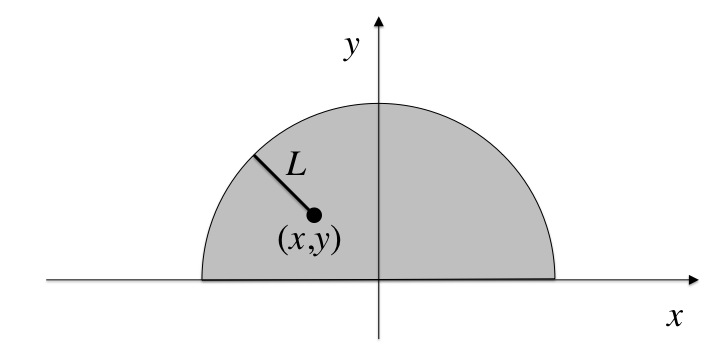
\includegraphics[width=0.65\textwidth]{ImgRadialCenterOfMass.jpg}
  \end{center}
 \begin{quote} \caption{\label{FigCircPlate}\small{The density of the plate at $(x,y)$ is equal to $L$.}}\end{quote}
\end{figure}
% ~~~~~~~~~~~~~~~~~~~~~~~~~~~~~~~~~~~~~~~~~~~~~~~~~~~~~~~~~~~~~~~~~~~~~~~~~~~~~~~~~
\item % MOMENTS OF A CYLINDER
\Emph{Center of Mass of a 2D Plate, Radial Density Function} \\

% ~~~~~~~~~~~~~~~~~~~~~~~~~~~~~~~~~~~~~~~~~~~~~~~~~~~~~~~~~~~~~~~~~~~~~~~~~~~~~~~~~
\item % EVEN AND ODD
\rednote{I'll push this question to a midterm or final exam}\\
Determine the value of
\begin{align*}
  \mathop{\int_0^{\pi} \!\! \int_{-1}^1} x^4e^{x^2 + y^2}\sin(y) dydx.
\end{align*}
Do not use integration by parts.
% ~~~~~~~~~~~~~~~~~~~~~~~~~~~~~~~~~~~~~~~~~~~~~~~~~~~~~~~~~~~~~~~~~~~~~~~~~~~~~~~~~
\EEN % END OF SUBSECTION 





